\section{Campaign Management and Communication} \label{sec:management}

Here we cover the management structures in place for HSC PDR2 
this includes the groups and meetings like the change control for 
the pipeline version.

\subsection{Rubin Teams}

Science Pipelines, DM Middleware, Campaign Management (CM), and Data Production
were all involved in HSC PDR2 production.

\begin{enumerate}

\item Data Production


\begin{itemize}
\item Yusra AlSayyad -- Lead
\item Jennifer Adelman-McCarthy Pilot
\item Brian Yanny co-Pilot
\end{itemize}


\item Campaign Management

\begin{itemize}
\item Eric Charles -- Lead
\item Orion Eiger
\item Sierra Villarreal
\item Fritz Mueller
\end{itemize}

\item Science Pipelines

\begin{itemize}
\item Yusra AlSayad - Science Pipelines 
\item Lauren MacArthur -- Science Pipelines
\item Eli Rykoff -- Photometric Calibration Pipeline Scientist
\end{itemize}

\item System Performance and V\&V

\begin{itemize}
\item Colin Slater - Lead Verification and Validation Scientist
\item Sophie Reed -- V\&V Analysis Tools
\end{itemize}

\item PanDA
\begin{itemize}
\item Wen Guan
\item Zhaoyu Yang
\end{itemize}

\item USDF infrastructure
\begin{itemize}
\item Wei Yang
\item Yee Li
\end{itemize}

\end{enumerate}

\subsection{Coordination}

The Data Production Lead defines campaigns (input datasets, software stack version, set of
steps (of pipetasks) to run, and rough deadline) to be run 
here: \url{https://confluence.lsstcorp.org/display/DM/Campaigns}, and assigns pilots and co-pilots.
For the HSC PDR2 campaign, overall notes are kept here: \url{https://confluence.lsstcorp.org/display/DM/2023+Internal+HSC+PDR2+Reprocessing+at+the+USDF}.   As this dataset has been previously processed, it was useful
to reference the earlier reprocessing from 2020 to compare visit lists, tract lists and other notes:
\url{https://confluence.lsstcorp.org/display/DM/S20+HSC+PDR2+Reprocessing}.

During the production of HSC PDR2 weekly coordination meetings were held with the Data Production 
and V\&V leads, the pilots, PanDA experts, and Middleware and CM developer reps. 

\subsection{Work Management}

We used Jira to track work related to the HSC PDR2 campaign.
%Epics and milestones were created in the \texttt{DM} Jira Project.
The main ticket was \jira{DM-39132} with linked subtickets for each step.
These tickets contained processing notes, and special situations that came up.

The slack channel {\it\#ops-cm-team} was used for questions and discussion as issues arose.
The channel {\it\#dm-hsc-reprocessing} was also a valuable resource as weekly processing of small
sets of HSC data were discussed here.

\subsection{Change Control Decisions during processing}

The Science Pipelines team working with V\&V and middleware determined which weekly release to use as a base
software distribution for the v24 stack.  Some tickets subsequent to the initial v24 stack branching
were backported into the v24 branch.  PDR2 used v24.1.0.rc2 for steps 1, 2a and 2b.

During processing, the Science Pipelines team continued to monitor progress and determine if updates were
needed to the software while processing.

The stack was updated to v24.1.0.rc3 for step 2c and beyond to incorporate an updated fgcm (photometric
calibration map covering the whole HSC PDR2 footprint) \jira{DM-39342}.

During the running of step3 and step7 two hot fixes were incorporated into processing, making use
of the CM '$\rm custom\_lsst\_setup$' feature, which allowed a github branch of code, along with a EUPS setup
file, to be loaded for processing on top of the base v24.1.0.rc3 stack.

The first hot fix was to the $\rm meas\_algorithms$ module to enable more robust dynamic sky estimation in very
crowded fields -- without this fix, large sections of the UDEEP tracts simply had no good detections or
measurements due to lack of sky objects.

The second hot fix was to the healSparse module to enable healSparsePropertyMaps (a step3 pipetask) and 
consolidateHealSparsePropertyMaps (step7) to proceed in cases where a tract or patch was not complete.
This allowed the HSC PDR2 propertyMap production to proceed even for tracts which were 
not completely filled in. These propertyMaps are need to make figures such as Figure \ref{fig:footprint0}.

We note that it was determined while applying these fixes that the stack setup and all 
hotfixes setup to generate the quantum graph for processing needs to be identical to 
the stack setups used to process the quantum graph.  This required changes to the 
job submission shell scripts and templates that CM uses for slurm quantum 
graph generation and running.   Multi-site processing should also be aware of this requirement.

\subsection{Production Hardware, Middleware, PanDA Workflow system, and SLURM USDF cluster}

\begin{itemize}

\item The basic node for DRP processing is a Linux box with 512 GB RAM and
128 cores (4GB/core).  The USDF has approximately 100 such nodes for
a total of 16K cores, however only about 3K were used during PDR2 to avoid
exceeding messaging limits between the PanDA DOMA system based at CERN 
and the USDF cluster at SLAC.  Future processing will use a local
PanDA installation at SLAC.  
		
\item The USDF nodes are managed by a SLURM batch
processing system which allocates resources according to core, memory and 
wallclock runtime requests.  The head nodes for the USDF cluster are 
known as sdfrome001 and sdfrome002.  For the first part of PDR2
processing the PanDA 'harvester' daemon, which distributes jobs between the
PanDA Queues and the SLURM managed worker nodes was located on the sdfrome001/2
head nodes.  This resulted in one instance of PanDA overload when the user load
on the head nodes became too large.  The PanDA harvester has since been
moved onto its own dedicated Virtual Machine (VM).

\item The Middleware used was a large gen-3 butler repository hosted
at the USDF.   The Campaign Management tools are used to 
generate data queries of reasonable size to 
request processing of groups of exposures or tracts
through steps of pipetasks.  The BPS interface
takes a bps yaml file of a group, generates a
quantum graph and execution butler for this
task and sends information for finding the graph
and execution butler on to PanDA for execution.
As outputs are generated by the worker nodes, references are 
temporarily gathered into a local execution butler.
Following the completion of all of a graphs tasks,
the local execution butler is merged back into
the main /repo/main butler at USDF.
Output tables, images, logs and metadata are 
also available in a large POSIX disk file system
at the USDF.

\item PanDA \url{https://panda.lsst.io/index.html} is the workflow 
management system used for the HSC PDR2 2023 campaign.
A set of daemons based at CERN, the PanDA DOMA test setup, accepted quantum
graphs of jobs,  sometimes consisting of hundreds of thousands of individual
quanta, and distributed them to worker nodes for execution.
\end{itemize}

Panda has a set of queue with different numbers of slots, memory limits and wallclock timeouts. 
One may view the number of jobs currently running in each queue here:
\url{https://panda-doma.cern.ch/dash/region} (auth required, increase Show entries from 20 to 50)
A Pull mode queue means there is a pilot job running on a worker node which pulls jobs to it from PanDA and
can handle large numbers of jobs per pilot.  A Push mode queue means that there is only one pilot per
job (usually for very long running or high memory jobs).   PanDA queue specifications used for
HSC PDR2 are listed in Table \ref{tab:pandaqueues}.

\normalsize 
\begin{center}
\begin{longtable}{|l|r|r|r|r|l|} 
\caption{PanDA Queue Names, Sizes, Time limits} \label{tab:pandaqueues}\\
\hline 
\textbf{Name}&\textbf{Slots}&\textbf{Memory}&\textbf{Wallclock}&\textbf{Push/Pull}&\textbf{Notes} \\ 
\hline
$\rm SLAC\_Rubin\_Merge$ & 200 & $<16$ GB & 24h & Push & MergeExecutionButler \\
$\rm SLAC\_Rubin$ & 4000 & $<4$ GB & 24h & Pull & 600 jobs/pilot \\
$\rm SLAC\_Rubin\_Medium$ & 3000 & $4-8$ GB & 24h & Pull &  600 jobs/pilot\\
$\rm SLAC\_Rubin\_Himem$ & 2500& $8-18$ GB & 24h & Pull &  600 jobs/pilot \\
$\rm SLAC\_Rubin\_Extra\_Himem$ & 1500 & $>18$ GB & 96h & Push & 1 job/pilot \\
\hline
\end{longtable} 
\end{center}
\normalsize

\subsection{Campaign Management}

Campaign Management \url{https://github.com/lsst-dm/cm_tools}, maintains a small sqlLite 
database of the heirarchy of campaign, step, group, workflow and job specifications for a production.
Both the pilot and co-pilot for a campaign can update and query the campaign database and use it to
drive generation of, and launch, and relaunch, bps submit yaml files to the panDA workflow system.

A set of templates defined in a local instance of the cm prod 
github repo \url{https://github.com/lsst-dm/cm_prod/tree/tickets/DM-39392/src/lsst/cm/prod/configs/PDR2} contains information about how to divide a large set of
exposures (step 1, 2, 4, 6) or tracts (step 3, 5) into groups of managable size for submission to PanDA.
Managable size is defined to be: quantum graph generates for a group in no more than about 1 hour and runtime
for a group is no more than about 6 hours in most cases.

The cm prod instance also contains working values of requestMemory for each pipetask to prevent
memory overflow and clustering directives for aggregating related pipetasks together so that they 
run as one job within panDA to reduce panDA messaging traffic.

CM generates automatically bps submit yaml files for each group for each step of a campaign.

There is a one-to-one relation between a cm job launch sent to PanDA for execution and a bps submit yaml file.

Because jobs may fail for production reasons (memory overflow, network glitch, scratch space overflow,
wallclock overflow), a workflow level of processing is defined, and a particular group of visits or tracts
may be resubmitted for processing multiple times, either as a 'rescue' 
(where a new workflow is defined as results from the previous workflow's progress are 
saved and added to), or as simply a 'requeue' of a workflow as a new
job (where the previous results are ignored and not collected at the end of
all groups' running for that step).

Typical use cases of the CM tools are documented at 
\url{https://confluence.lsstcorp.org/display/DM/CM+Tools+usage+notes}.

As the CM tools are under active development, there were several times during PDR2 production where the CM
prod database needed to be adjusted by hand to mark a complete and consistent set of output collections
that could be gathered together by a chain collection operation in the butler to produce a single 
collection in the butler for each PDR2 step.  I.E. The tagged collection 
\code{$\rm HSC/runs/PDR2/v24\_1\_0/DM-39132/step3$} contains entries from step3 processing of 
all 710 tracts in the PDR2 outputs. The order of the collections matters since in a few cases, 
the outputTable datasetTypes needed to be rerun to fix an
issue with missing data.  So long as one uses the --find-first switch when querying 
the collection for analysis, this returns complete and unique dataset entries.

\subsection{DRP Processing Scaling and Timing estimates}

LSST survey metrics such as typical exposures per night, data volumes
object counts and survey depth are given at 
\url{https://confluence.lsstcorp.org/pages/viewpage.action?spaceKey=LKB&title=LSST+Key+Numbers}.

From these one may estimate that the roughly 17K exposures and 500 
square degrees of the HSC PDR2 tract coadds is roughly 3\% of an 
early year DRP with typically 400K exposures and 6000 tracts 
over 18,000 square degrees.

Annual processing is scheduled to fit into an approximately 200 day window
for each annual DRP.

Thus to process 3\% of a DRP, one has about 200*0.03 = 6 days wallclock time
to reduce a dataset the size of PDR2.

Figure \ref{fig:cores} shows the average core usage over the first
three steps of processing.  Not counting a schedule downtime 
over July 4, the wallclock times for steps 1, 2 and 3 extended over
17d, 20d and 27days respectively.

\begin{figure}
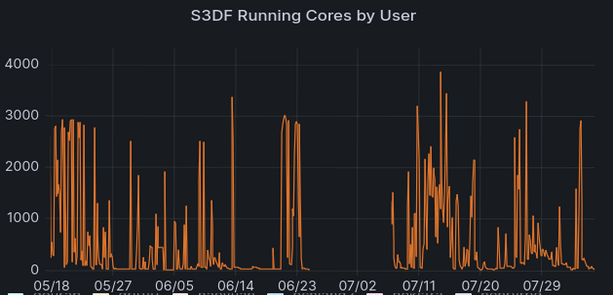
\includegraphics[width=0.9\textwidth]{Campcorespdr2.png}
\caption{Cores in use in PDR2 step1,step2,step3 campaign.}  \label{fig:cores}
\end{figure}

To date (Aug 2023), it took 64 days wallclock time to get through 
steps 1,2 and 3 with a 3,000 core cluster at USDF.  
Steps 4, 5 and 6 and Q/A plots are estimated to take approximately 
16 days more, or 80 days for all of PDR2.   This is roughly a 
factor of 80/6 = 13 too long.

Increasing the number of cores by a factor of three with multisite processing
leaves a factor of four in improvement still required.
As is clear from Fig. \ref{fig:cores}, far less than the available 3K cores
were in use for most of the duration -- the cores were not used
efficiently.

Some of the apparent inefficiency was due to running jobs with memory
settings greater than the minimum of 4GB/job, and this reduces the available
cores by the factor by which the requested memory per job exceeds 4GB.
For instance, if one runs jobs in the himem queue, requesting 16GB/job,
then only 3000/4 = 750 cores are available in the USDF cluster.

This is not the primary reason, however, for the inefficient use of cores.
Much more common issues during this HSC PDR2 processing was the 
experimentation required to  determine the correct requestMemory and clustering
settings required for each pipetask in each step.

While some guidance was known ahead of time from weekly reprocessing
campaigns, since those campaigns only typically involved a few tracts and
a few hundred exposures, scaling estimates could not always be made
in advance.

Trial and error, with successive memory increases and sometimes the need to
reduce clustering to avoid memory overflows was needed during each of
steps 1, 2b, 2c, 2e, 3 runs, costing several weeks of lost efficiency.

Additionally, issues with overflowing scratch space on the worker nodes,
contention for resources between the panDA harvester and user jobs on the 
USDF head nodes and networking hiccups or queue sizing inefficiencies 
with PanDA also required several days each to track down and correct.

All that said, much of the experience gained from this exercise are
now captured in the requestMemory.yaml and clustering.yaml files
in \url{https://github.com/lsst-dm/cm_prod/tree/tickets/DM-39392/src/lsst/cm/prod/configs/PDR2} repository, along with processing notes at:
\url{https://confluence.lsstcorp.org/display/DM/2023+Internal+HSC+PDR2+Reprocessing+at+the+USDF}, so that should HSC PDR2 be run again, in multi-site 
mode using a total of approximately 10K cores, it should be 
possible to reduce overall wallclock time to close to the desired 6 days,
provided data transfer between sites is efficiently handled.

Known inefficienies in some science pipeline codes can also be made to
reduce memory usage of several pipetasks (i.e. \jira{DM-38772}).
